\section{experiments}
\begin{table}[t]%[htbp]
\centering
\scriptsize
%\tiny
\caption{\label{tab_Data} Statistics of the four datasets. %The first row of each dataset corresponds to the number of users, items and interactions. 
The last column reports the selected meta-paths in each dataset. }
{
\begin{tabular}{c||c|c|c|c|c}
\hline
Datasets & {Relations (A-B)} & {\#A} & {\#B} & {\#A-B} & Meta-paths\\
%{} & {(A-B)} & {of A} & {of B} & {of (A-B)} & {}\\
\hline
\hline
\multirow{4}{*}{Movielens} & {\emph{User-Movie}} & {943} & {1,682} & {100,000}   & {\emph{UMUM}}\\
\cline{2-5}
\multirow{4}{*}{} &  {User-Age} & {943} & {8} & {943}    & {\emph{UMGM}}\\
\cline{2-5}
\multirow{4}{*}{} &{User-Occupation} & {943} & {21} & {943}  & {\emph{UAUM}}\\
\cline{2-5}
\multirow{4}{*}{} & {Movie-Genre} & {1,682} & {18} & {2,861}   & {\emph{UOUM}}\\
\hline
\hline
\multirow{4}{*}{LastFM} & {\emph{User-Artist}} & {1,892} & {17,632} & {92,834}  & {\emph{UATA}} \\
\cline{2-5}
\multirow{4}{*}{} & {User-User} & {1,892} & {1,892} & {18,802}   & {\emph{UAUA}}\\
\cline{2-5}
\multirow{4}{*}{} & {Artist-Artist} & {17,632} & {17,632} & {153,399}   & {\emph{UUUA}}\\
\cline{2-5}
\multirow{4}{*}{} & {Artist-Tag} & {17,632} & {11,945} & {184,941}   & {\emph{UUA}}\\
\hline
\hline
\multirow{4}{*}{Yelp} & {\emph{User-Business}} & {16,239} & {14,284} & {198,397}   & {\emph{UBUB}}\\
\cline{2-5}
\multirow{4}{*}{} & {User-User} & {16,239} & {16,239} & {158,590}  & {\emph{UBCaB}} \\
\cline{2-5}
\multirow{4}{*}{} & {Business-City (Ci)} & {14,267} & {47} & {14,267}  & {\emph{UUB}} \\
\cline{2-5}
\multirow{4}{*}{} & {Business-Category (Ca)} & {14,180} & {511} & {40,009}   & {\emph{UBCiB}}\\
\hline
\hline
\multirow{4}{*}{Amazon} & {\emph{User-Item}} & {3,584} & {2,753} & {50,903}   & {\emph{UIUI}}\\
\cline{2-5}
\multirow{4}{*}{} & {Item-View} & {2,753} & {3857} & {5,694}  & {\emph{UIVI}} \\
\cline{2-5}
\multirow{4}{*}{} & {Item-Brand} & {2,753} & {334} & {2,753}  & {\emph{UIBI}} \\
\cline{2-5}
\multirow{4}{*}{} & {Item-Category} & {2,753} & {22} & {5,508}   & {\emph{UICI}}\\
\hline
\end{tabular}}
\end{table}

\begin{table*}[t]
\centering
\small
\caption{\label{tab_Effectiveness} Results of effectiveness experiments on four datasets. We use ``*'' to mark the best performance from the baselines.} %for each comparison.}
{
\begin{tabular}{c||c|c||c|c||c|c||c|c}
\hline
\multirow{2}{*}{Models}&
\multicolumn{2}{c||}{Movielens}& \multicolumn{2}{c||}{LastFM} & \multicolumn{2}{c||}{Yelp} & \multicolumn{2}{c}{Amazon}\\
\cline{2-9}
  & {HR@10}&{NDCG@10} & {HR@10}&{NDCG@10} & {HR@10}&{NDCG@10} & {HR@10}&{NDCG@10}\\
\hline
\hline
{ItemKNN} & {0.5854} & {0.3368} & {0.6327} & {0.5176} & {0.1480} & {0.0944} & {0.3153} & {0.1864}\\
\hline
{BRP}  & {0.6766*} & {0.3860} & {0.7690} & {0.6061} & {0.5162} & {0.3186} & {0.3890} & {0.2195}\\
\hline
{MF}  & {0.6702} & {0.3869*} & {0.7611} & {0.6051} & {0.5139} & {0.3176} & {0.3379} & {0.1893}\\
\hline
{NeuMF}  & {0.6723} & {0.3816} & {0.7579} & {0.6070*} & {0.6660*} & {0.4218*} & {0.3619} & {0.2023}\\
\hline
{LRML}  & {0.6140} & {0.3500} & {0.7204} & {0.5411} & {0.5934} & {0.3608} & {0.3304} & {0.1788}\\
\hline
{SVDFeature$_{hete}$}  & {0.6033} & {0.3366} & {0.7848*} & {0.5813} & {0.6586} & {0.4117} & {0.3111} & {0.1575}\\
\hline
{FMG$_{rank}$}  & {0.6267} & {0.3519} & {0.7758} & {0.5905} & {0.6080} & {0.3418} & {0.4154*} & {0.2244*}\\
\hline
\hline
{LGRec$_{noAtt}$}  & {0.4836} & {0.2446} & {0.7104} & {0.5531} & {0.1372} & {0.0756} & {0.2720} & {0.1380}\\
\hline
{LGRec$_{noGlo}$}  & {0.6564} & {0.3824} & {0.7717} & {0.6060} & {0.5894} & {0.3353} & {0.3820} & {0.2151}\\
\hline
{LGRec}  & {\textbf{0.6914}} & {\textbf{0.3989}} & {\textbf{0.7865}} & {\textbf{0.6228}} & {\textbf{0.6902}} & {\textbf{0.4396}} & {\textbf{0.4235}} & {\textbf{0.2383}}\\
\hline
\end{tabular}}
\end{table*}
\paratitle{Datasets and evaluation metrics.} We evaluate our proposed model over four real-world datasets, namely MovieLens
%\footnote{http://grouplens.org/datasets/movielens/}
, LastFM
%\footnote{http://www.last.fm}
, Yelp~\cite{hu2018leveraging}
%\footnote{http://www.yelp.com/dataset-challenge}
 and Amazon\footnote{http://jmcauley.ucsd.edu/data/amazon/}, The detailed descriptions of the four datasets are summarized in Table~\ref{tab_Data}.
%\paratitle{Evaluation metrics.} 
We adopt the widely used leave-one-out method to evaluate the performance of item recommendation~\cite{he2017neural,tay2018latent}. For each golden item (\eg the item user has interacted with) in the test, we randomly sample 100 negative items and rank the golden item among the 100 items. Following~\cite{he2017neural}, we adopt Hit ratio at rank $k$ (HR@$k$) and Normalized Discounted Cumulative Gain at rank $k$ (NDCG@$k$) to evaluate the performance of model performance.

\paratitle{Compared methods.} We consider the following representative recommendation methods for performance comparisons. (1) \emph{ItemKNN}: It is a typical collaborative filtering method by recommending similar items based on past items~\cite{sarwar2001item}; (2) \emph{BPR}: It optimizes the MF model with the pairwise ranking loss~\cite{rendle2009bpr}; (3) \emph{MF}: It optimizes the classical MF model with the cross entropy loss~\cite{he2017neural}; (4) \emph{NeuMF}: It is the recently proposed neural network method for top-$N$ recommendation~\cite{he2017neural}; (5) $LRML$: It is the state-of-the-art memory based attention model for item recommendation~\cite{tay2018latent}; (6) \emph{SVDFeature$_{hete}$}: We extract heterogeneous information as one-hot feature to feed into \emph{SVDFeature} for recommendation~\cite{chen2012svdfeature}; (7) \emph{FMG$_{rank}$}: It is the state-of-the-art HIN based recommendation by optimizing the pair ranking loss~\cite{zhao2017meta}.

%It is noteworthy that our model it is flexible to integrate neighborhood information and heterogeneous information based relation. 
To examine the effectiveness of the co-attention mechanism and the global information modeling method, we consider two variants as compared baselines, namely LGRec$_{noAtt}$ (our model without co-attention mechanism) and LGRec$_{noGlo}$ (our model without global information). And LGRec is our complete model.

%\paratitle{Implementation details.}
%We implement the proposed model based on Tensorflow. For our model, we randomly initialize model parameters with Gaussion distribution and utilize Adam~\cite{kingma2014adam} as the optimizer, and set the batch size as 256. The learning rate is tuned amongst \{0.0001, 0.0005, 0.001\}. The margin $\lambda$ is tuned amongst \{0.1, 0.5, 1.0, 2.0\}. And we set $K_1 = K_2 = 100$, $\alpha = 0.1$, $\beta = 0.001$ and the embedding dimension to 128. For HIN based methods, we use the meta-paths reported in Table~\ref{tab_Data}. For \emph{MF} and \emph{NeuMF}, we follow the optimal configuration and architecture reported in~\cite{he2017neural}. For the other comparison methods, we optimize their parameters using 10\% training data as the validation set.


\paratitle{Results and analysis.}
We report the comparison results of our proposed model and baselines on four datasets in Table~\ref{tab_Effectiveness}. The major findings from the experimental results are summarized as follows: (1) LGRec is consistently better than all the baselines on the four datasets. This observation demonstrates the effectiveness of our model on the task of top-$N$ recommendation, which is more capable of utilizing local neighborhood information and global heterogenous information. (2) Considering the two variants of LGRec, we can find that the overall performance order is as follows: LGRec $>$ LGRec$_{noGlo}$ $>$ LGRec$_{noAtt}$. The result indicates that the gobal information and co-attention mechanism really work in our model and the global information play a critical role for the performance improvement in most cases. (3) Among these baselines, HIN based methods (SVDFeature$_{hete}$ and FMG$_{rank}$) outperform CF methods (ItemKNN, BPR and MF) in most cases, which indicates the usefulness of heterogeneous information. %Besides, NeuMF is a competitive methods among these baselines, which benefits from the nonlinearity of multi-layer perceptron.
In addition, NeuMF also  achieves competitive performance due to the adoption of neural network, while its performance is still worse than LGRec because of the absence of heterogeneous information.

\paratitle{Parameter tuning.}
We examine the effect of balance parameter $\alpha$ and the dimension of embeddings $d$ on the performance for our model. As shown in Fig~\ref{fig-para}, we can see that (1) when $\alpha = 0.1$, our model achieves the best performance, indicating that the balance parameter should be set to a small number; and (2) our model achieves the best performance when $d = 128$, which indicates that the dimension of embeddings cannot be set too small or too large.

\begin{figure}[htbp]
\centering
\subfigure[Varying $\alpha$]{
\begin{minipage}[t]{0.45\linewidth}
\centering
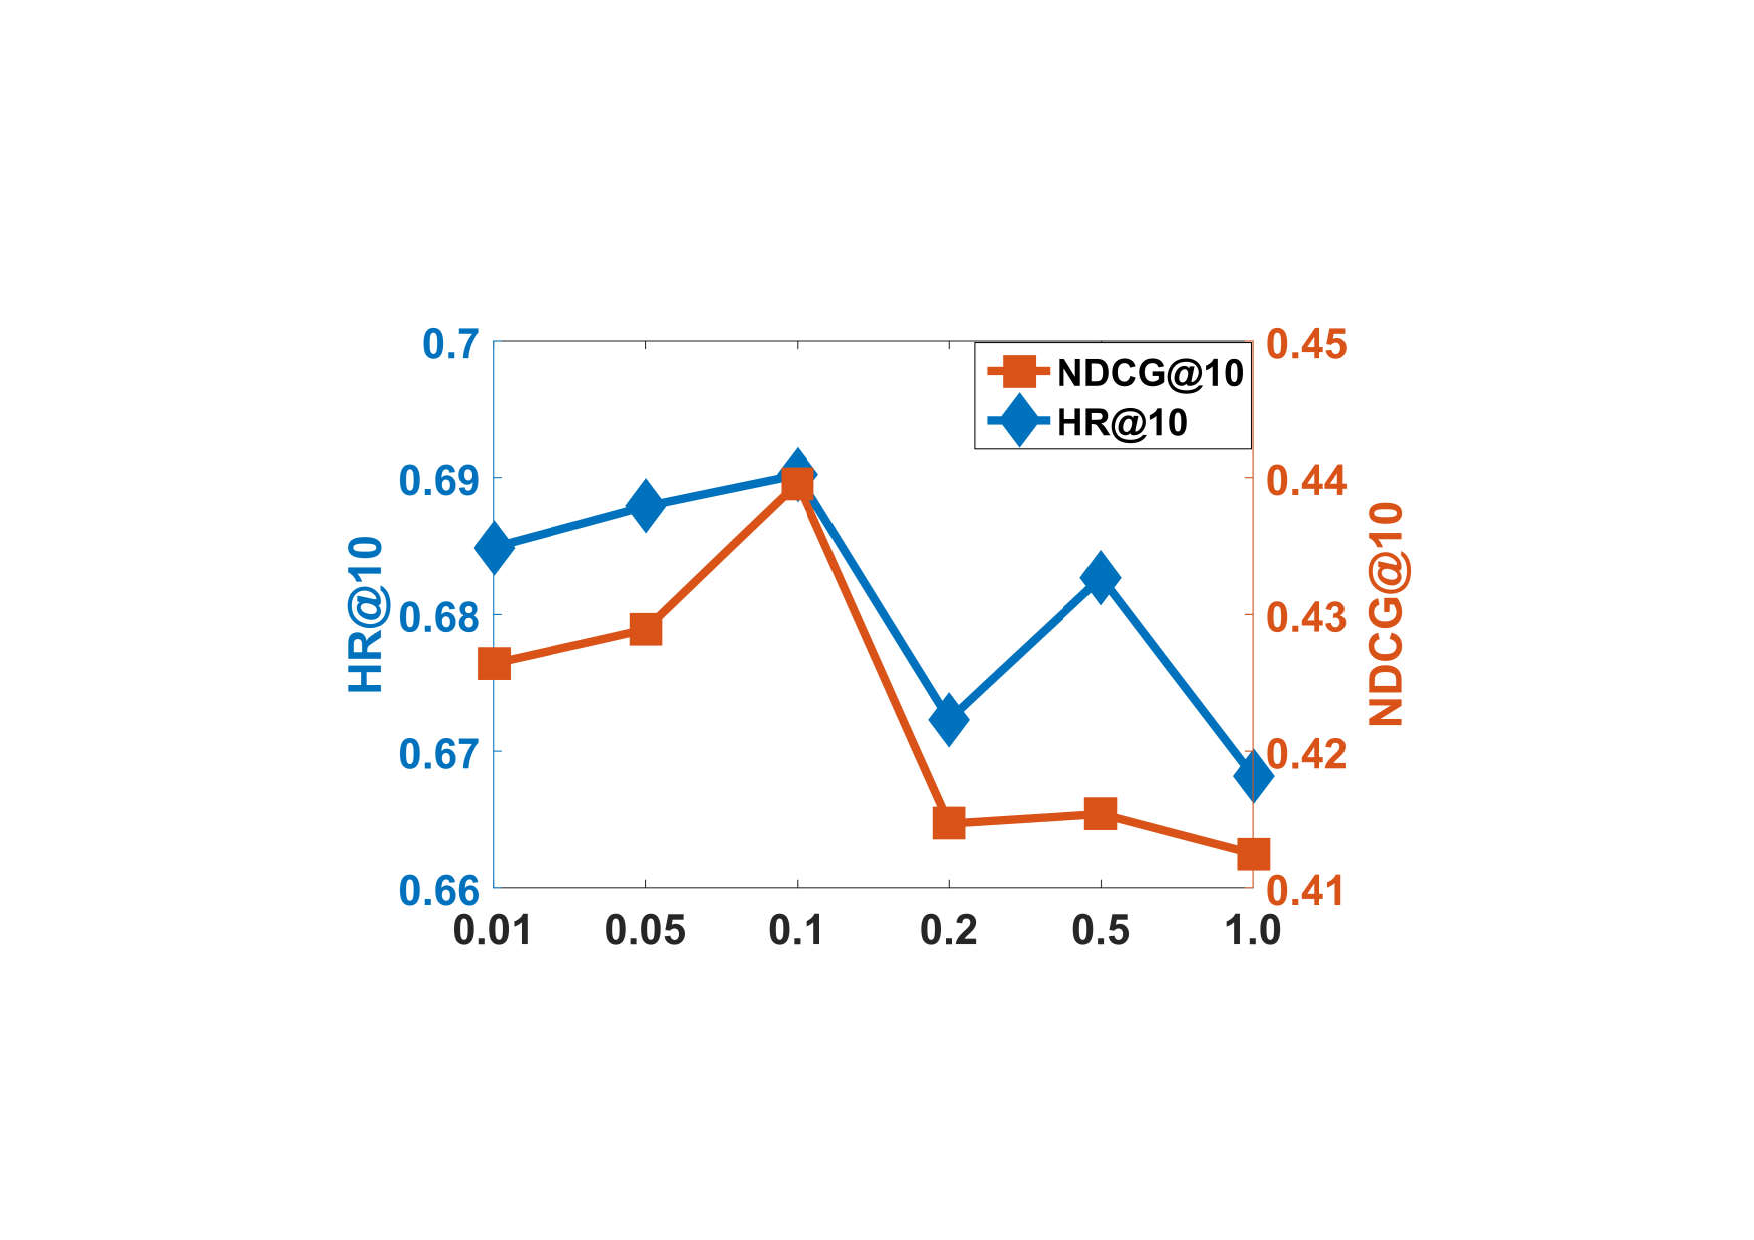
\includegraphics[width=4cm]{image/alpha_yelp.pdf}
\end{minipage}
}
%\hspace{30pt}
\subfigure[Varying $d$]{
\begin{minipage}[t]{0.45\linewidth}
\centering
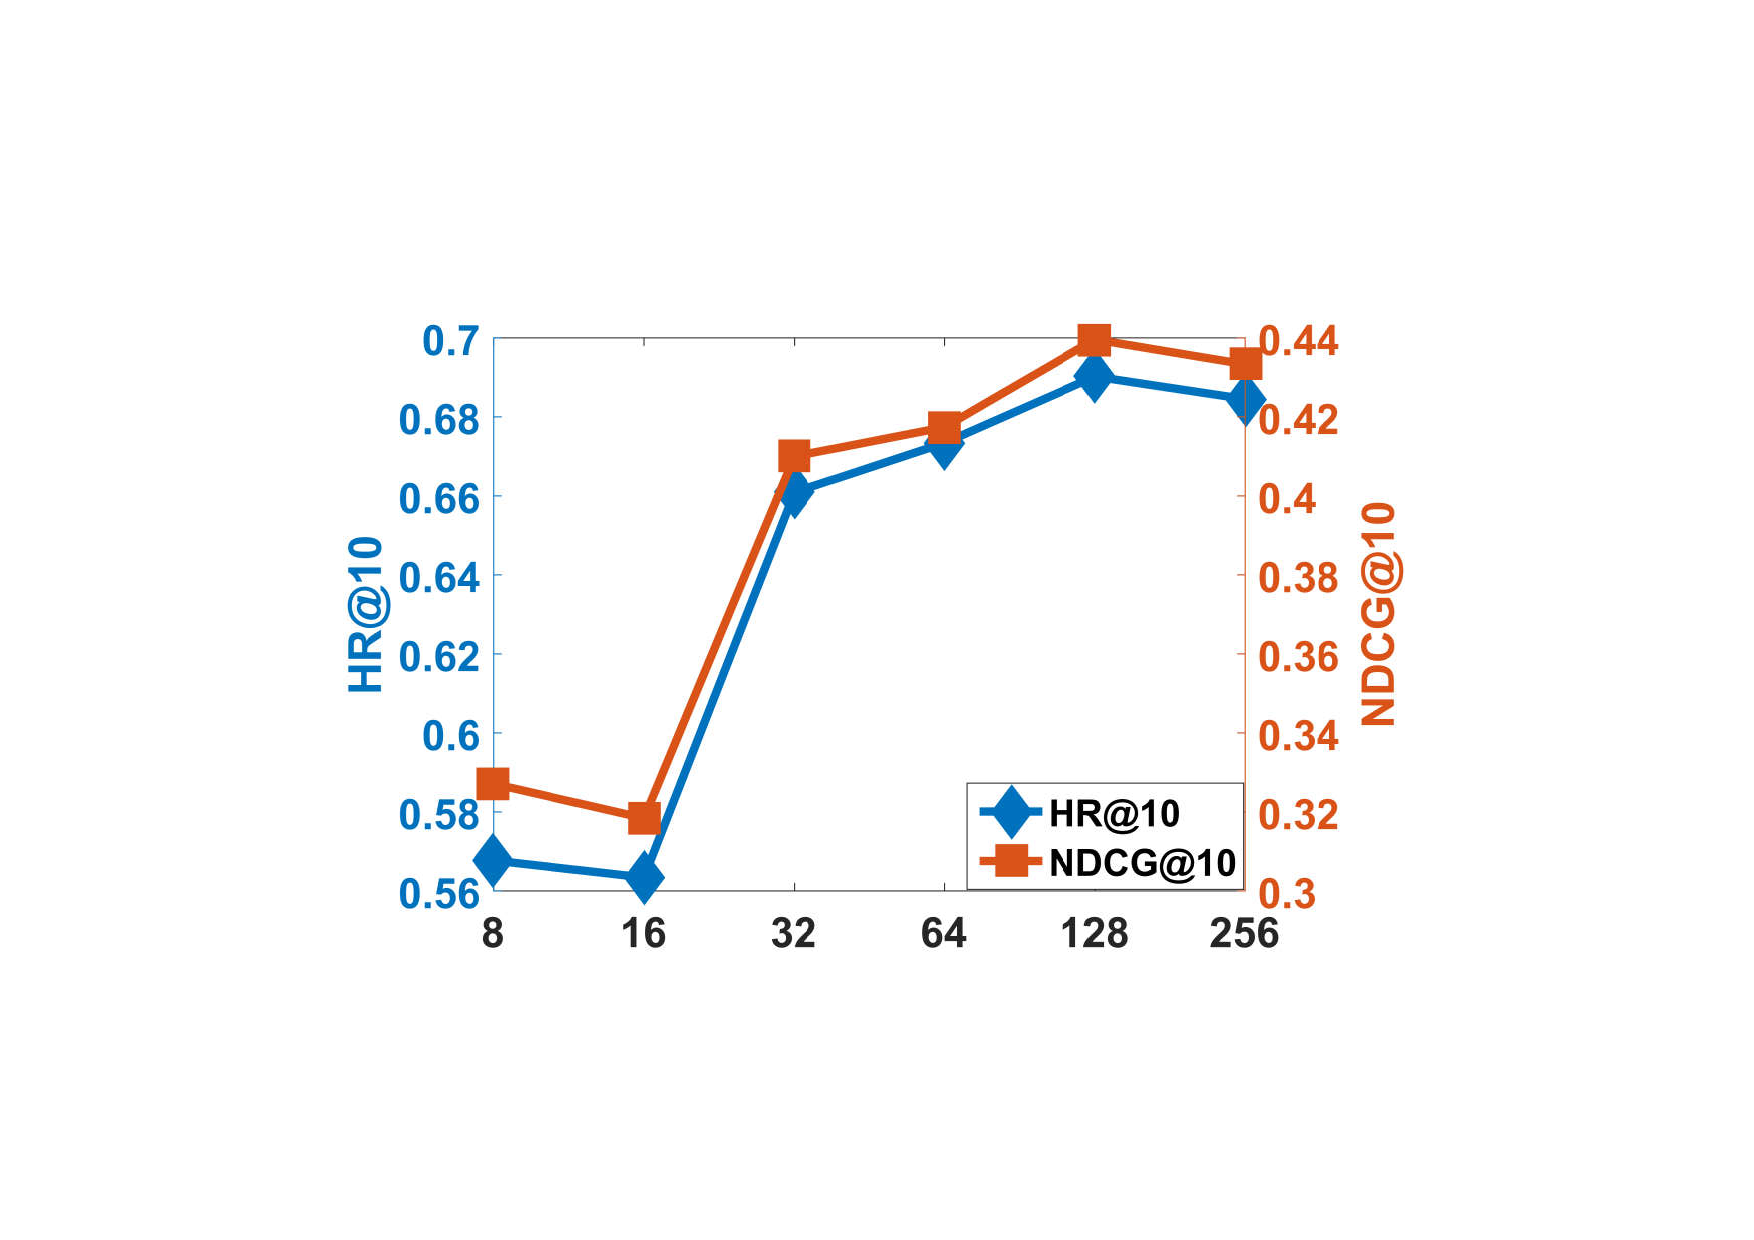
\includegraphics[width=4cm]{image/dim_yelp.pdf}
\end{minipage}
}
\caption{Performance tuning with the varying of the parameter $\alpha$ and the dimension of embeddings $d$ on Yelp dataset.\label{fig-para}}
\end{figure}
